\documentclass[12pt]{article}
\usepackage{graphicx}
\usepackage{xspace}
\usepackage{color, colortbl}
\usepackage{amssymb}
\pagestyle{empty}
\definecolor{Gray}{gray}{0.9}
\textwidth      165mm
\textheight     240mm
\topmargin      -18mm
\oddsidemargin  -2mm
\evensidemargin 2mm
\newcommand{\impl}{\mathbin{\Rightarrow}}
\newcommand{\biim}{\mathbin{\Leftrightarrow}}
\renewcommand{\theenumi}{\alph{enumi}}

\author{Emmanuel Macario - 831659}
\title{COMP30026 Models of Computation Assignment 1}
\date{September, 2018}

\begin{document}

\maketitle

\subsection*{Challenge 1}
\begin{enumerate}
\item 
$\begin{array}{|ccc|c|c|}
   \hline
   P & Q & R & ((\neg P \land Q) \impl \neg R) \impl R & R
\\ \hline
    0 & 0 & 0 & 0 & 0
\\ 0 & 0 & 1 & 1 & 1
\\ 0 & 1 & 0 & 0 & 0
\\ 0 & 1 & 1 & 1 & 1
\\ 1 & 0 & 0 & 0 & 0
\\ 1 & 0 & 1 & 1 & 1
\\ 1 & 1 & 0 & 0 & 0
\\ 1 & 1 & 1 & 1 & 1
\\ \hline
\end{array}$
$\therefore ((\neg P \land Q) \impl \neg R) \impl R \equiv R$
\bigskip

\item 
$\begin{array}{|ccc|c|c|}
   \hline
   P & Q & R & (P \impl (Q \lor R)) \land (P \biim Q) & P \biim Q
\\ \hline
    0 & 0 & 0 & 1 & 1
\\ 0 & 0 & 1 & 1 & 1
\\ 0 & 1 & 0 & 0 & 0
\\ 0 & 1 & 1 & 0 & 0
\\ 1 & 0 & 0 & 0 & 0
\\ 1 & 0 & 1 & 0 & 0
\\ 1 & 1 & 0 & 1 & 1
\\ 1 & 1 & 1 & 1 & 1
\\ \hline
\end{array}$
$\therefore (P \impl (Q \lor R)) \land (P \biim Q) \equiv P \biim Q$
\bigskip

\item
$\begin{array}{|cc|c|c|}
   \hline
   P & Q & P \impl (P \biim Q) & P \impl Q
\\ \hline
    0 & 0 & 1 & 1
\\ 0 & 1 & 1 & 1
\\ 1 & 0 & 0 & 0
\\ 1 & 1 & 1 & 1
\\ \hline
\end{array}$
$\therefore P \impl (P \biim Q) \equiv P \impl Q$
\bigskip

\item
$\begin{array}{|ccc|c|c|}
   \hline
   P & Q & R & P \lor (R \impl Q) & (Q \impl P) \impl (R \impl P)
\\ \hline
    0 & 0 & 0 & 1 & 1
\\ 0 & 0 & 1 & 0 & 0
\\ 0 & 1 & 0 & 1 & 1
\\ 0 & 1 & 1 & 1 & 1
\\ 1 & 0 & 0 & 1 & 1
\\ 1 & 0 & 1 & 1 & 1
\\ 1 & 1 & 0 & 1 & 1
\\ 1 & 1 & 1 & 1 & 1
\\ \hline
\end{array}$
$\therefore P \lor (R \impl Q) \equiv (Q \impl P) \impl (R \impl P)$
\bigskip

\end{enumerate}


\subsection*{Challenge 2}

Firstly, let us define both inhabitant's statements in propositional logic.
Inhabitant $P$'s statements are equivalent to $\neg Q$ and $Q'$, respectively. 
Inhabitant $Q$'s statements are equivalent to $P$ and $\neg P'$, respectively.

\bigskip
\noindent
We are given information that the statements given by the inhabitants $P$ and $Q$ 
respectively must be either true or false, but \emph{cannot} be a mixture of both. 
In other words, if an inhabitant lies, then every statement they say is guaranteed to 
be a false statement.

\bigskip
\noindent
This means that if inhabitant $P$ is telling the truth, then $\neg Q \land Q'$ is true, 
otherwise $Q \land \neg Q'$ must be true. Similarly, if inhabitant $Q$ is telling the truth,
then $P \land \neg P'$ must be true, otherwise $\neg P \land P'$ must be true.


\bigskip
\noindent
Let $A$ mean $P$ \emph{is telling the truth}, and $B$ mean $Q$ is \emph{telling
the truth}. We can surmise when $P$ and $Q$ are lying or telling the truth via truth tables.

\bigskip
\begin{minipage}{0.5\textwidth}
\begin{center}
$\begin{array}{|cc|c|}
   \hline
   P & P' & A
\\ \hline
   0 & 0 & 1
\\ 0 & 1 & 0
\\ 1 & 0 & 0
\\ 1 & 1 & 1
\\ \hline
\end{array}$
\end{center}
\end{minipage}
\begin{minipage}{0.35\textwidth}
\begin{center}
$\begin{array}{|cc|c|}
   \hline
   Q & Q' & B
\\ \hline
   0 & 0 & 1
\\ 0 & 1 & 0
\\ 1 & 0 & 0
\\ 1 & 1 & 1
\\ \hline
\end{array}$
\end{center}
\end{minipage}

\bigskip
\noindent
It can be seen that $P$ is truthful when $P \biim P'$ is true, and lies when $P 
\oplus P'$ is true. The same notions hold for inhabitant $Q$, with respect to 
literals $Q$ and $Q'$.

\bigskip
\noindent
Using the formulas generated above, we can now extract the maximal amount of information 
provided by the two  inhabitants, in the form of propositional formulas (1) and (2), both of which
must be true.

\medskip
\begin{equation}
((P \biim P') \land (\neg Q \land Q')) \oplus ((P \oplus P') \land (Q \land \neg Q'))
\end{equation}
\begin{equation}
((Q \biim Q') \land (P \land \neg P')) \oplus ((Q \oplus Q') \land (\neg P \land P'))
\end{equation}

\bigskip
\noindent
Using a truth table, we can determine for each of $P$ and $Q$ whether they 
are a knight or a knave, and whether they are healthy or sick.

\bigskip
\begin{center}
\resizebox{0.95\textwidth}{!}{$\begin{array}{|cccc|c|c|}
   \hline
   P & P' & Q & Q' & ((P \biim P') \land (\neg Q \land Q')) \oplus ((P \oplus P') \land (Q \land \neg Q')) & 
   ((Q \biim Q') \land (P \land \neg P')) \oplus ((Q \oplus Q') \land (\neg P \land P'))
\\ \hline
   0 & 0 & 0 & 0 & 0 & 0 
\\ 0 & 0 & 0 & 1 & 1 & 0
\\ 0 & 0 & 1 & 0 & 0 & 0
\\ 0 & 0 & 1 & 1 & 0 & 0 
\\ 0 & 1 & 0 & 0 & 0 & 0 
\\ 0 & 1 & 0 & 1 & 0 & 1 
\\ \rowcolor{Gray}
   0 & 1 & 1 & 0 & 1 & 1 
\\ 0 & 1 & 1 & 1 & 0 & 0
\\ 1 & 0 & 0 & 0 & 0 & 1 
\\ 1 & 0 & 0 & 1 & 0 & 0 
\\ 1 & 0 & 1 & 0 & 1 & 0 
\\ 1 & 0 & 1 & 1 & 0 & 1 
\\ 1 & 1 & 0 & 0 & 0 & 0 
\\ 1 & 1 & 0 & 1 & 1 & 0 
\\ 1 & 1 & 1 & 0 & 0 & 0 
\\ 1 & 1 & 1 & 1 & 0 & 0
\\ \hline
\end{array}$}
\end{center}

\bigskip
\noindent
We know that both formulas must be true. Therefore,
there is only \emph{one} possible scenario. That is, $P$
is a \emph{healthy knave} and $Q$ is a \emph{sick knight}.

% CHALLENGE 3
\subsection*{Challenge 3}
\begin{enumerate}
  \item
Consider the interpretation $I$ with domain $D$ = \{0,1\} and $P(0)$. Additionally, 
let $Q$ always be \emph{false}.

\bigskip
\noindent
For this interpretation, it can be seen that $I \vDash \forall x
(P(x)) \impl Q$, but $I \nvDash \forall x(P(x) \impl Q)$.
Hence, $\forall x(P(x)) \impl Q \nvDash \forall x(P(x) \impl Q)$.

\bigskip
\noindent
Therefore, $\forall x (P(x)) \impl Q$ is \emph{not} equivalent to
$\forall x(P(x) \impl Q)$.

\bigskip
\item We can prove this by re-writing the LHS formula into the RHS formula, shown below.

\begin{center}
\begin{tabular}{l r}
$\exists x(Q \impl R(x))$ & \textbf{Original LHS}\\
$\equiv \exists x(\neg Q \lor R(x))$ & \textbf{Eliminate $\impl$}\\
$\equiv \exists x(\neg Q) \lor \exists x(R(x))$ & \textbf{Distribute $\exists x$ over $\lor$}\\
$\equiv \neg Q \lor \exists x(R(x))$ & \textbf{Since $Q$ is a formula with no free occurrences of $x$}\\
$\equiv Q \impl \exists x(R(x))$ & \textbf{Rewrite $\neg A \lor B$ into $A \impl B$}\\
\end{tabular}
\end{center}

$\therefore \exists x(Q \impl R(x)) \equiv Q \impl \exists x(R(x))$ 

\end{enumerate}


% CHALLENGE 4
\subsection*{Challenge 4}
\begin{enumerate}
  \item $\forall x \forall y(M(x,y) \impl F(x))$
  \item $\forall x \forall y((U(x) \land M(y,x)) \impl U(y))$
  \item $\forall x((F(x) \land U(x) \land B(x)) \impl D(x))$
  \item $\forall x \forall y((U(x) \land M(x,y) \land D(x)) \impl D(y))$
  \item $\forall x((S(x) \land U(x)) \impl B(x))$
\end{enumerate}

\bigskip
\noindent
For each formula, a \emph{Horn clause} can be easily generated by negating the antecedent and
eliminating the implication, then pushing in the negation, and eliminating all universal quantifiers. The 
set of \emph{Horn clauses} generated are as follows:

\begin{enumerate}
  \item $\{\neg M(x,y), F(x)\}$
  \item $\{\neg U(x), \neg M(y,x), U(y)\}$
  \item $\{\neg F(x), \neg U(x), \neg B(x), D(x)\}$
  \item $\{\neg U(x), \neg M(x,y), \neg D(x), D(y)\}$
  \item $\{\neg S(x), \neg U(x), B(x)\}$
\end{enumerate}

\bigskip
\noindent
Let us express statement (f) in first-order predicate logic.

\bigskip
f.  $\forall x \forall y((U(x) \land M(y,x) \land S(y)) \impl D(x))$

\bigskip
\noindent
The negation of (f) in clausal form is: 

$\neg \forall x \forall y((U(x) \land M(y,x) \land S(y)) \impl D(x))$

$\rightsquigarrow \exists x \neg \forall y((U(x) \land M(y,x) \land S(y)) \impl D(x))$

$\rightsquigarrow \exists x \exists y(U(x) \land M(y,x) \land S(y) \land \neg D(x))$

$\rightsquigarrow \exists y(U(a) \land M(y,a) \land S(y) \land \neg D(a))$

$\rightsquigarrow U(a) \land M(b,a) \land S(b) \land \neg D(a)$

\bigskip
\noindent
Which produces \emph{four} clauses: 

$\{U(a)\}, \{M(b,a)\}, \{S(b)\}, \{\neg D(a)\}$

\bigskip
\noindent
Now, we can find a refutation of the set of nine clauses.

\begin{center}
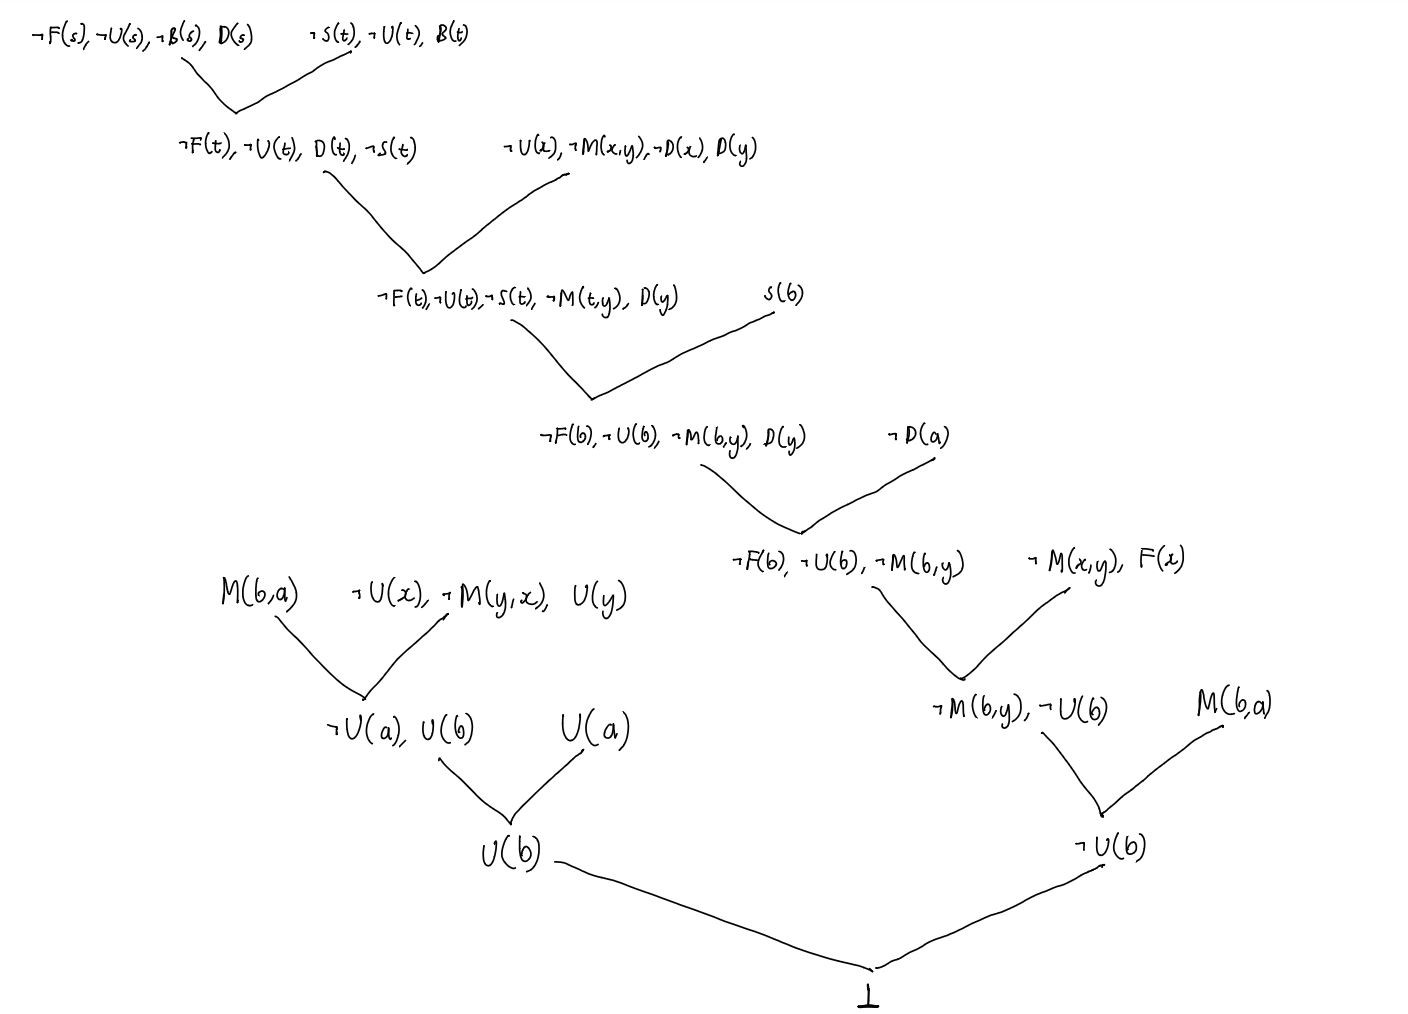
\includegraphics[width=6in,height=5in,keepaspectratio]{q4_refutation.jpg}
\end{center}

\bigskip
\noindent
By the refutation proof shown above, we have shown that the conjunction of
premise statements (a)-(e) and the negation of conclusion statement (f) is
unsatisfiable. 

\bigskip
\noindent
$\therefore$ (f) is a logical consequence of statements (a)-(e)



% CHALLENGE 5
\subsection*{Challenge 5}

\begin{enumerate}
  \item The statements expressed in first-order predicate logic are as follows:\\\\
	  (a1) $\forall x \forall y(N(x,y) \impl N(y,x))\\\\$
        (a2) $\forall x \forall y (\exists u(M(u,x) \land \neg M(u,y)) \impl N(x,y))\\\\$
        (a3) $\forall x(\neg \exists u(M(u,x)) \impl E(x))\\\\$
        (a4) $\forall x \forall y \forall u((D(x,y) \land M(u,x)) \impl \neg M(u,y))$\\

  \item The set of clauses produced by statements (a1)-(a4) are as follows:\\
\\(a1) $\{N(x,y), N(y,x)\}$\\
\\(a2) $\{\neg M(u,x), M(u,y), N(x,y)\}$\\
\\(a3) $\{M(f(x), x), E(x)\}$\\
\\(a4) $\{\neg D(x,y), \neg M(u,x), \neg M(u,y)\}$

  \bigskip
  \item Firstly, we must transform the fifth statement into first-order predicate logic. The statement is equivalent to the formula $\forall x \forall y(D(x,y) \impl (N(x,y) \lor (E(x) \land E(y))))$.

\bigskip
Since we would like to use this formula in a refutation proof as the logical consequence of other statements, we must negate it and then convert its negation to clausal form.

\bigskip
The negation of the statement in clausal form is equal to:

$\neg \forall x \forall y(D(x,y) \impl (N(x,y) \lor (E(x) \land E(y))))$

$\rightsquigarrow \exists x \neg \forall y(D(x,y) \impl (N(x,y) \lor (E(x) \land E(y))))$

$\rightsquigarrow \exists x \exists y(\neg (D(x,y) \impl (N(x,y) \lor (E(x) \land E(y)))))$

$\rightsquigarrow \exists x \exists y(\neg (D(x,y) \impl (N(x,y) \lor (E(x) \land E(y)))))$

$\rightsquigarrow \exists x \exists y(D(x,y) \land \neg (N(x,y) \lor (E(x) \land E(y)))))$

$\rightsquigarrow \exists x \exists y(D(x,y) \land ((\neg N(x,y) \land \neg E(x)) \lor (\neg N(x,y) \land \neg E(y))))$

$\rightsquigarrow \exists x \exists y((D(x,y) \land \neg N(x,y) \land \neg E(x)) \lor (D(x,y) \land \neg N(x,y) \land \neg E(y)))$

$\rightsquigarrow \exists x \exists y(D(x,y) \land \neg N(x,y) \land (\neg E(x) \lor \neg E(y)))$

$\rightsquigarrow D(a,b) \land \neg N(a,b) \land (\neg E(a) \lor \neg E(b))$

\bigskip
Hence, the fifth statement produces \emph{three} clauses:

$\{D(a,b)\}, \{\neg N(a,b)\}, \{\neg E(a), \neg E(b)\}$

\bigskip
\item Refutation Proof:
\end{enumerate}

\begin{center}
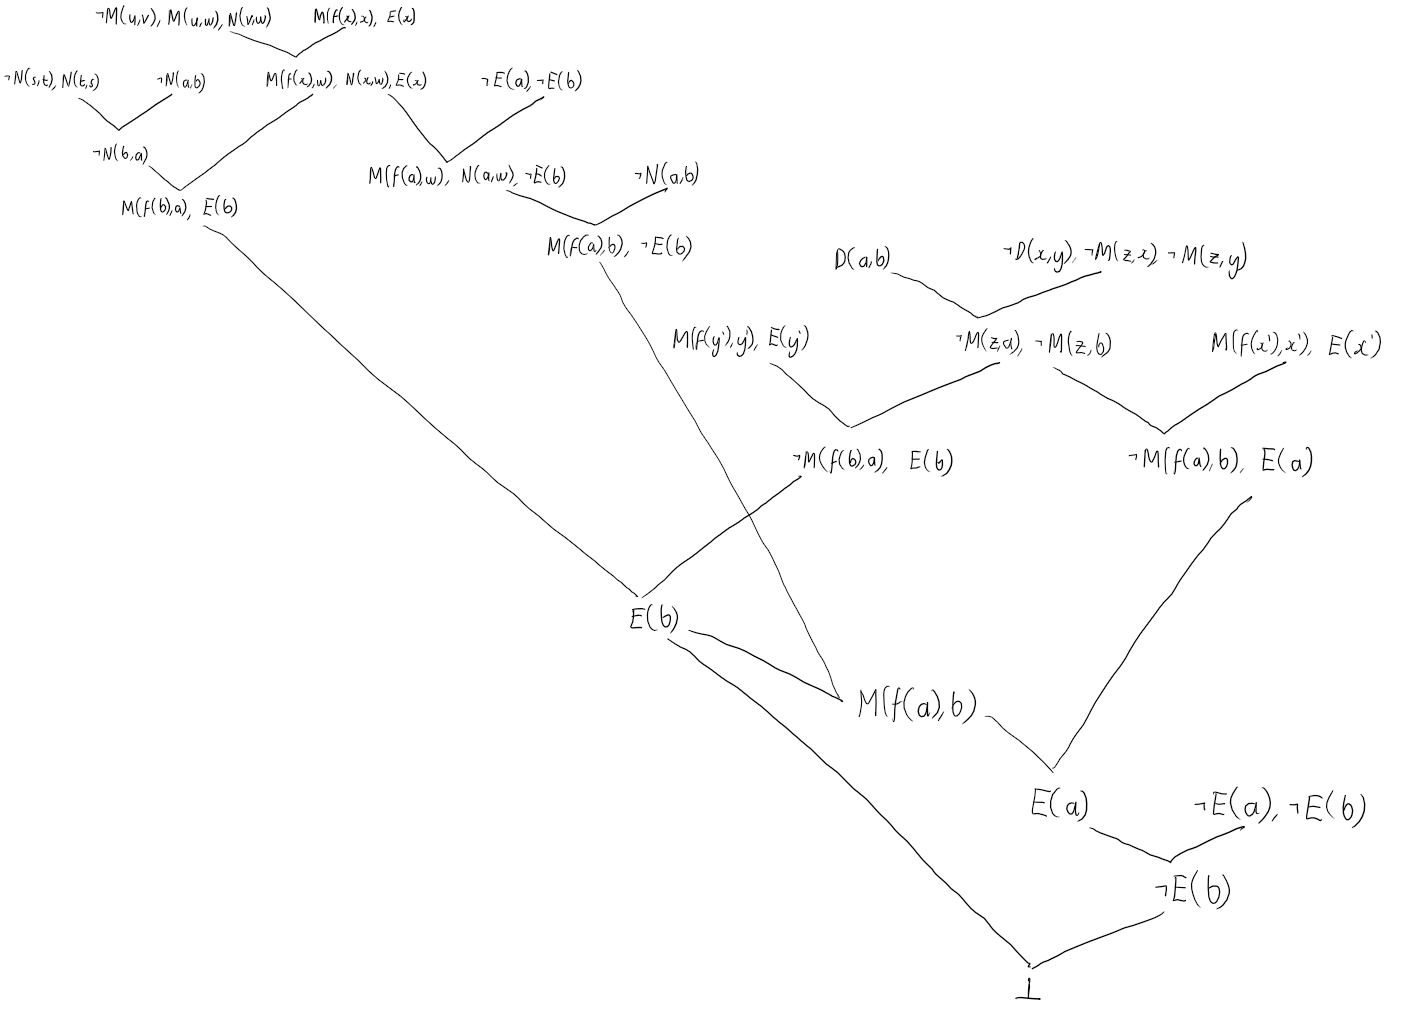
\includegraphics[width=7in,height=6in,keepaspectratio]{q5_refutation.jpg}
\end{center}

\bigskip
\noindent
By the refutation proof shown above, we have shown that the conjunction of
premise statements (a1)-(a4) and the negation of conclusion statement is
unsatisfiable.
\bigskip
\noindent

$\therefore$ The fifth statement is entailed by statements (a1)-(a4).

% CHALLENGE 6
\subsection*{Challenge 6}
See Grok.


\end{document}